\section{DA Wandler\hartl{455}}

\subsection{Parallelverfahren (Voltage Scaling)}

\renewcommand{\arraystretch}{1}
\begin{tabular}{|>{\bfseries}p{3cm}|c|p{6.6cm}|}
	\hline
	Strom-DAC \hartl{456} 
	& 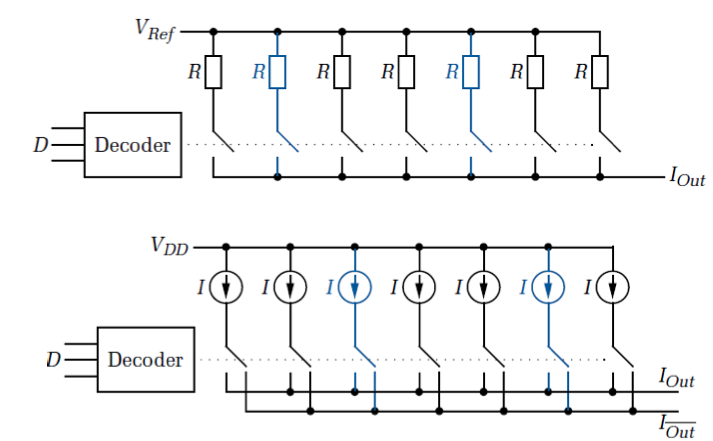
\includegraphics[width=7cm, valign=t]{pictures/Strom-DAC}
	& {\begin{align*}
		K &=2^N-1\\
		I &=\frac{V_{Ref}}{R}\\
		I_{Out} &=D \cdot I=D\cdot\frac{V_{Ref}}{R}\\
		I_{Out} &=D \cdot I\\
		I_{\bar{Out}} &=(K-D)\cdot I\\
		V_{Out} &=RI_{Out}-RI_{\bar{Out}} \\
			    &=(D-K)\cdot RI	
	  \end{align*}}
	  \begin{tabular}{lp{5cm}}
	  	K: & Anzahl Stromquellen \\
      	D: & Eingangswert (Anzahl Schalter die aktiv sind.)
      \end{tabular}
	\\ \hline
	String DAC \hartl{459}
	& 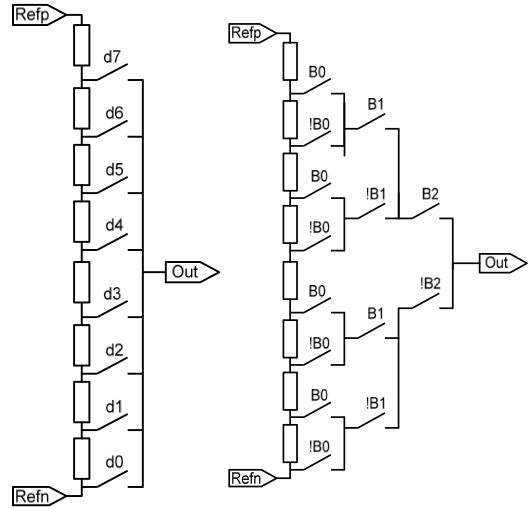
\includegraphics[width=5.5cm, valign=t]{pictures/string_DAC}
	& 
		\begin{description}
  		\item[Vorteile: ] garantierte Stetigkeit
  		\item[Nachteile:] benötigt $2^n$ Widerstände und $2^n$ Schalter, n-to-$2^n$ Decoder(linke Variante)
	  \end{description}
	  {\begin{align*}
	  	V_{Out_{ideal}}(D)=\frac{D}{2^n}(V_{Ref+}-V_{Ref-})+V_{Ref-}\\
	  	V_{Out_{real}}(D)=V_{Ref-}+\left(V_{Ref+}-V_{Ref-}\right)\cdot\\
	  	\cdot\frac{D*R_{Load}}{2^n*R*D-R*D^2+2^n*R_{Load}+2^n*R_{Switch}}\\
	  	DAC_{error}(D)=\frac{V_{out_{real}}(D)-V_{out_{ideal}}(D)}{V_{out_{ideal}}(D)}\\
	  \end{align*}}
	  
	\\ \hline
	Segmented String DAC \hartl{459}
	& 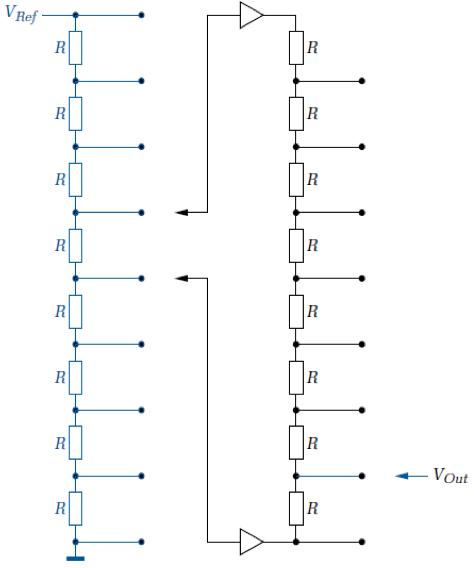
\includegraphics[width=5cm, valign=t]{pictures/segmented_string_DAC}
	& \begin{description}
  		\item[Vorteile: ] viel weniger Elemente
  		\item[Nachteile:] benötigt Buffer (offset-frei)
	  \end{description}
	\\ \hline
	Digitales Potentiometer \hartl{460}
	& 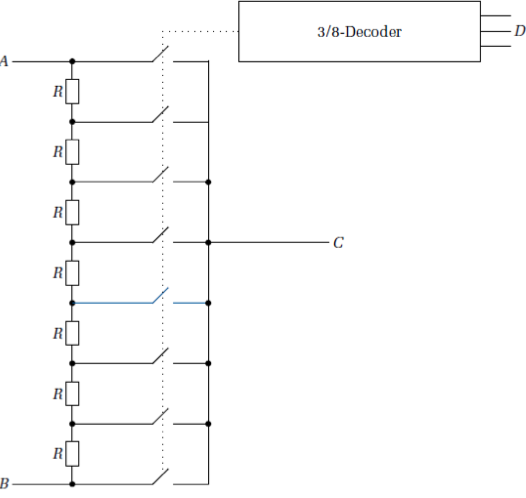
\includegraphics[width=5cm, valign=t]{pictures/digitales_potentiometer}
	& \begin{description}
  		\item[Vorteile: ] automatisierter Elektronik-Test möglich
	  \end{description}
	\\ \hline
\end{tabular}
\renewcommand{\arraystretch}{\arraystretchOriginal}

\subsection{Wägeverfahren\hartl{461}} 
\begin{longtable}{|>{\bfseries}p{3cm}|c|p{8.6cm}|}
	\hline
	Spannungs"-summierung \hartl{461}
	& 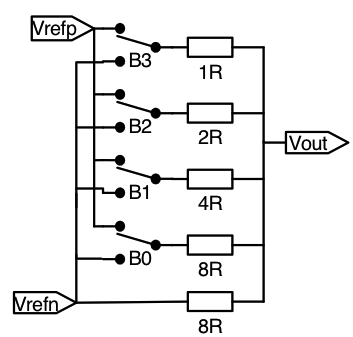
\includegraphics[width=5cm, valign=t]{./pictures/spannungssummierung.png}
	& {\begin{align*}
		V_{Out} &= \frac{B0 \cdot 2^0 \cdot G0+B1 \cdot 2^1 \cdot G0}{2^4 \cdot G0} \\
				& \quad \cdot \frac{B2 \cdot 2^2 \cdot G0+B3 \cdot 2^3 \cdot G0}{2^4 \cdot G0}\\
		        & \quad \cdot (V_{rep}-V_{refn})+V_{refn}
	  \end{align*}}
	  \begin{description}
  		\item[Vorteile:] N Widerstände, N Schalter
  		\item[Nachteile:] nicht garantiert stetig, grosse Wertebereiche für Widerstände, rechnen mit Leitwerten ($G_0 = \frac{1}{8R}$)
	  \end{description}
	\\ \hline
	Strom"-summierung \hartl{462}
	& 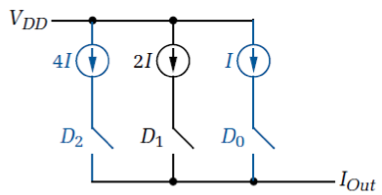
\includegraphics[width=4.5cm, valign=t]{./pictures/stromsummierung.png}
	& \begin{equation*}
		V_{Out}=(4+1) \cdot I
	  \end{equation*}
	\\ \hline
	Praktisch
	& 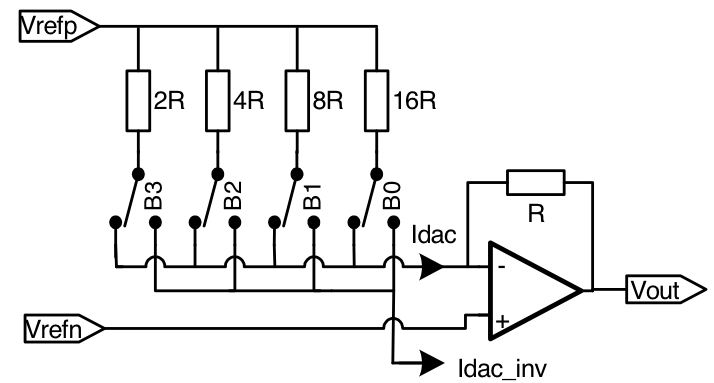
\includegraphics[width=6cm, valign=t]{./pictures/praktisch.png}
	& \[
		Idac_{max}=\frac{V_{refp}-V_{refn}}{R} \cdot \frac{2^n-1}{2^n}
	  \]
	\\ \hline
	R-2R-Netzwerk \hartl{462}
	& 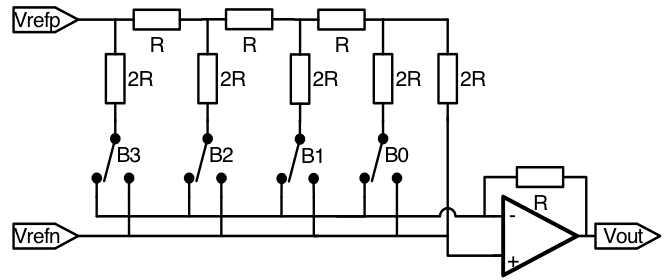
\includegraphics[width=6cm, valign=t]{./pictures/r2rnetzwerk.png}
	&
	\\ \hline
	Kapazitiver DAC
	& 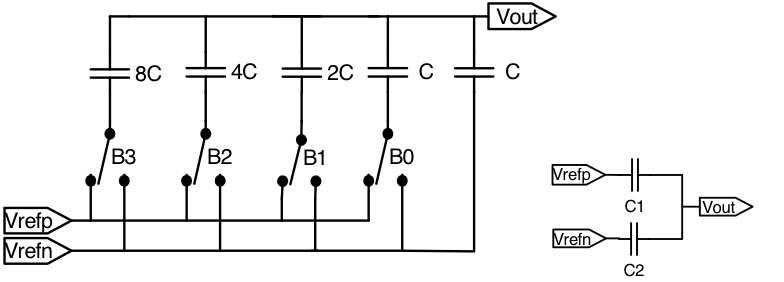
\includegraphics[width=6cm, valign=t]{./pictures/kapazitiverDAC.png}
	& {\begin{align*}
		C1	&= B3 \cdot 8C+B2 \cdot 4C+ B1 \cdot 2C+B0 \cdot C \\
		C2	&= !B3 \cdot 8C+!B2 \cdot 4C+ !B1 \cdot 2C+!B0 \cdot C+C \\
		V_{Out}& =\frac{C1}{C1+C2}\cdot (V_{refp}-V_{refn})\\
		\text{mit } & C1+C2=2^n\cdot C
	  \end{align*}}
	\\ \hline
\end{longtable}


\subsection{Zählverfahren(PWM)\hartl{466}}
\begin{longtable}{|>{\bfseries}p{4cm}|l|p{8cm}|}
	\hline 
	Grundprinzip \hartl{466}
	& 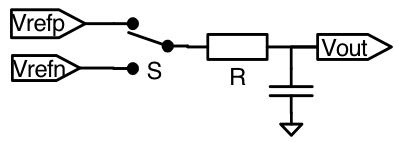
\includegraphics[width=6cm, valign=t]{./pictures/pwm_DAC.png}
	& $V_{Out}=\frac{D}{2^n} \cdot (V_{refp}-V_{refn})+V_{refn}$	  
	  \begin{description}
  		\item[Vorteile:] einfache Schaltung, hohe Auflösung, Funktioniert ohne analoge Schaltung onchip (z.B. mit FPGA, Microcontroller) 
  		\item[Nachteile:] sehr langsam, benötigt grosse Zeitkonstante (Kapazität offchip)
	  \end{description}
	\\ \hline
	PWM-Ansteuerung \hartl{466}
	& \parbox[c][2cm]{6cm}{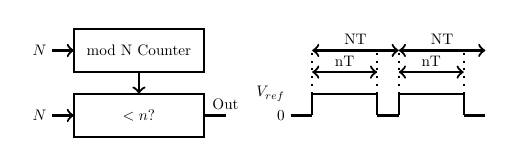
\begin{tikzpicture}[thick, transform shape, scale=0.55]
	\draw node at (0.5,0) [anchor=east] {$N$};
	\draw [->] (0.5,0) -- (1,0);
	\draw (1,0.5) rectangle (4,-0.5);
	\draw node at (2.5,0) {mod N Counter};
	
	\draw [->] (2.5,-0.5) -- (2.5,-1);
	
	\draw node at (0.5,-1.5) [anchor=east] {$N$};
	\draw [->] (0.5,-1.5) -- (1,-1.5);
	\draw (1,-1) rectangle (4,-2);
	\draw node at (2.5,-1.5) {$<n?$};
	
	\draw (4,-1.5) -- (4.5,-1.5) node [anchor=south] {Out};
	
	%PWM Signal:
	\node at (6,-1) [anchor=east] {$V_{ref}$};
	\node at (6,-1.5) [anchor=east] {$0$};
	
	\foreach \x in {6.5,8,8.5,10}
	{
		\draw (\x,-1) -- (\x,-1.5);
		\draw [dotted] (\x,-1) -- (\x,0);
	}
	\foreach \x in {6,8,10}
		\draw (\x,-1.5) -- (\x+0.5,-1.5);
	\foreach \x in {6.5,8.5}
		\draw (\x,-1) -- (\x+1.5,-1);
	
	\foreach \x in {6.5,8.5}
	{
		\draw [<->] (\x,0) -- (\x+2,0);
		\node at (\x+1,0) [anchor=south] {NT};
	}
	\foreach \x in {6.5,8.5}
	{
		\draw [<->] (\x,-0.5) -- (\x+1.5,-0.5);
		\node at (\x+0.75,-0.5) [anchor=south] {nT};
	}

\end{tikzpicture}}
	& $\bar{V_{Out}}=\frac{n}{N}V_{Ref}$
	  \begin{tabular}{ll}
		N:&Takte\\
		n:&digitale Eingangsgrösse
	  \end{tabular}
	\\ \hline
\end{longtable}


\subsubsection{Kaskadierte DAC}
\begin{longtable}{|>{\bfseries}p{4cm}|c|p{8cm}|}
	\hline
	Grundprinzip
	& 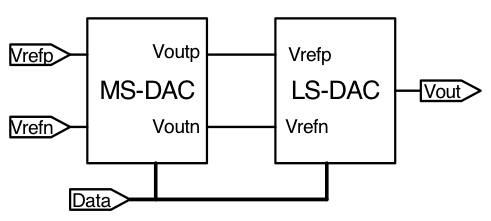
\includegraphics[width=6cm, valign=t]{./pictures/kaskadiertDAC.png}
	& \begin{itemize}
  		\item MS-DAC hat 2 Ausgangsspannungen (Über und unter dem gewünschten
  			$V_{Out}$)
  		\item LS-DAC hat kleine Eingangspannungsdifferenz $\to$ höhere Auflösung der
  			Spannung
	  \end{itemize}
	\\ \hline
	Zyklisch, algorithmischer DAC \hartl{466}
	& 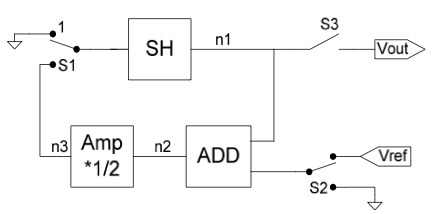
\includegraphics[width=6cm, valign=t]{./pictures/zyklischDAC.png}
	& \textbf{Ablauf der Wandlung}
	  \begin{enumerate}
  		\item Die Spannung im S/H löschen (Schalter S1), S3 offen)
  		\item S1 auf den Verstärker-Ausgang schalten
  		\item Laufvariale k wird auf 0 gesetzt
  		\item S2 setzen: VREF oder GND ( abh. $D_{K}$).
  		\item Der Addierer und Verstärker generieren Ausgangssignal
  		\item Im S/H wird die Feedback-Spannung gespeichert (S1)
  		\item X wird um 1 erhöht
  		\item Gehe zu Schritt 4, wenn $X\leq n$
	  \end{enumerate}
	\\ \hline
	Pipelined DAC 
	& 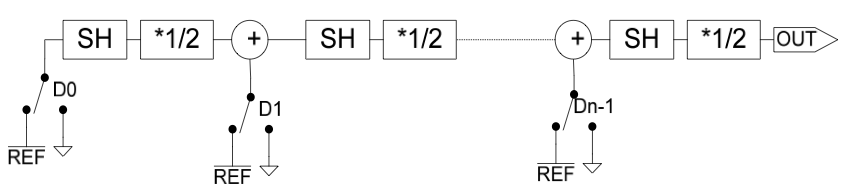
\includegraphics[width=6cm, valign=t]{pictures/piplinedDAC}
	& Die Latenz beträgt n Zyklen, die Update-Frequenz ist aber n-mal grösser
	\\ \hline
	Strom-DAC
	& 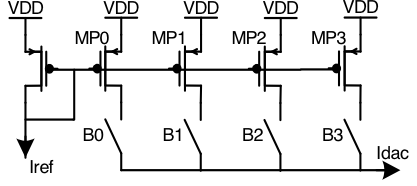
\includegraphics[width=6cm, valign=t]{pictures/stromDAC}
	& \begin{itemize}
  		\item Stromspiegel
  		\item MP0 ist gleich breit wie Stromquellen-MOS $\to$ I(MP0)=Iref
  		\item MP1 ist doppelt so breit wie MP0 $\to I(MP1)=2*Iref$
  		\item MP2 ist doppelt so breit wie MP1 $\to I(MP2)=4*Iref$
  		\item \ldots
	  \end{itemize}
	\\ \hline
\end{longtable}


\subsection{Multiplizierender DAC\hartl{470}} 

